\documentclass[12pt,a4paper]{book}
\raggedbottom

\usepackage{ugmath_notas}
\usepackage{float}
\usepackage{placeins}
\usepackage[labelfont=bf,labelsep=space]{caption}
\usepackage{pdfpages}
\usepackage{tikz-cd}
\usepackage{amsthm}
\renewcommand{\Tr}{\operatorname{Tr}}
\newcommand{\llaves}[1]{\{#1\}}
\newcommand{\parentesis}[1]{\left(#1\right)}
\newcommand{\corchetes}[1]{\left[#1\right]}
\newcommand{\llavesgrande}[1]{\big\{#1\big\}}
\newcommand{\llavesgrandes}[1]{\left\{#1\right\}}


\begin{document}
        
    
    \thispagestyle{empty}
    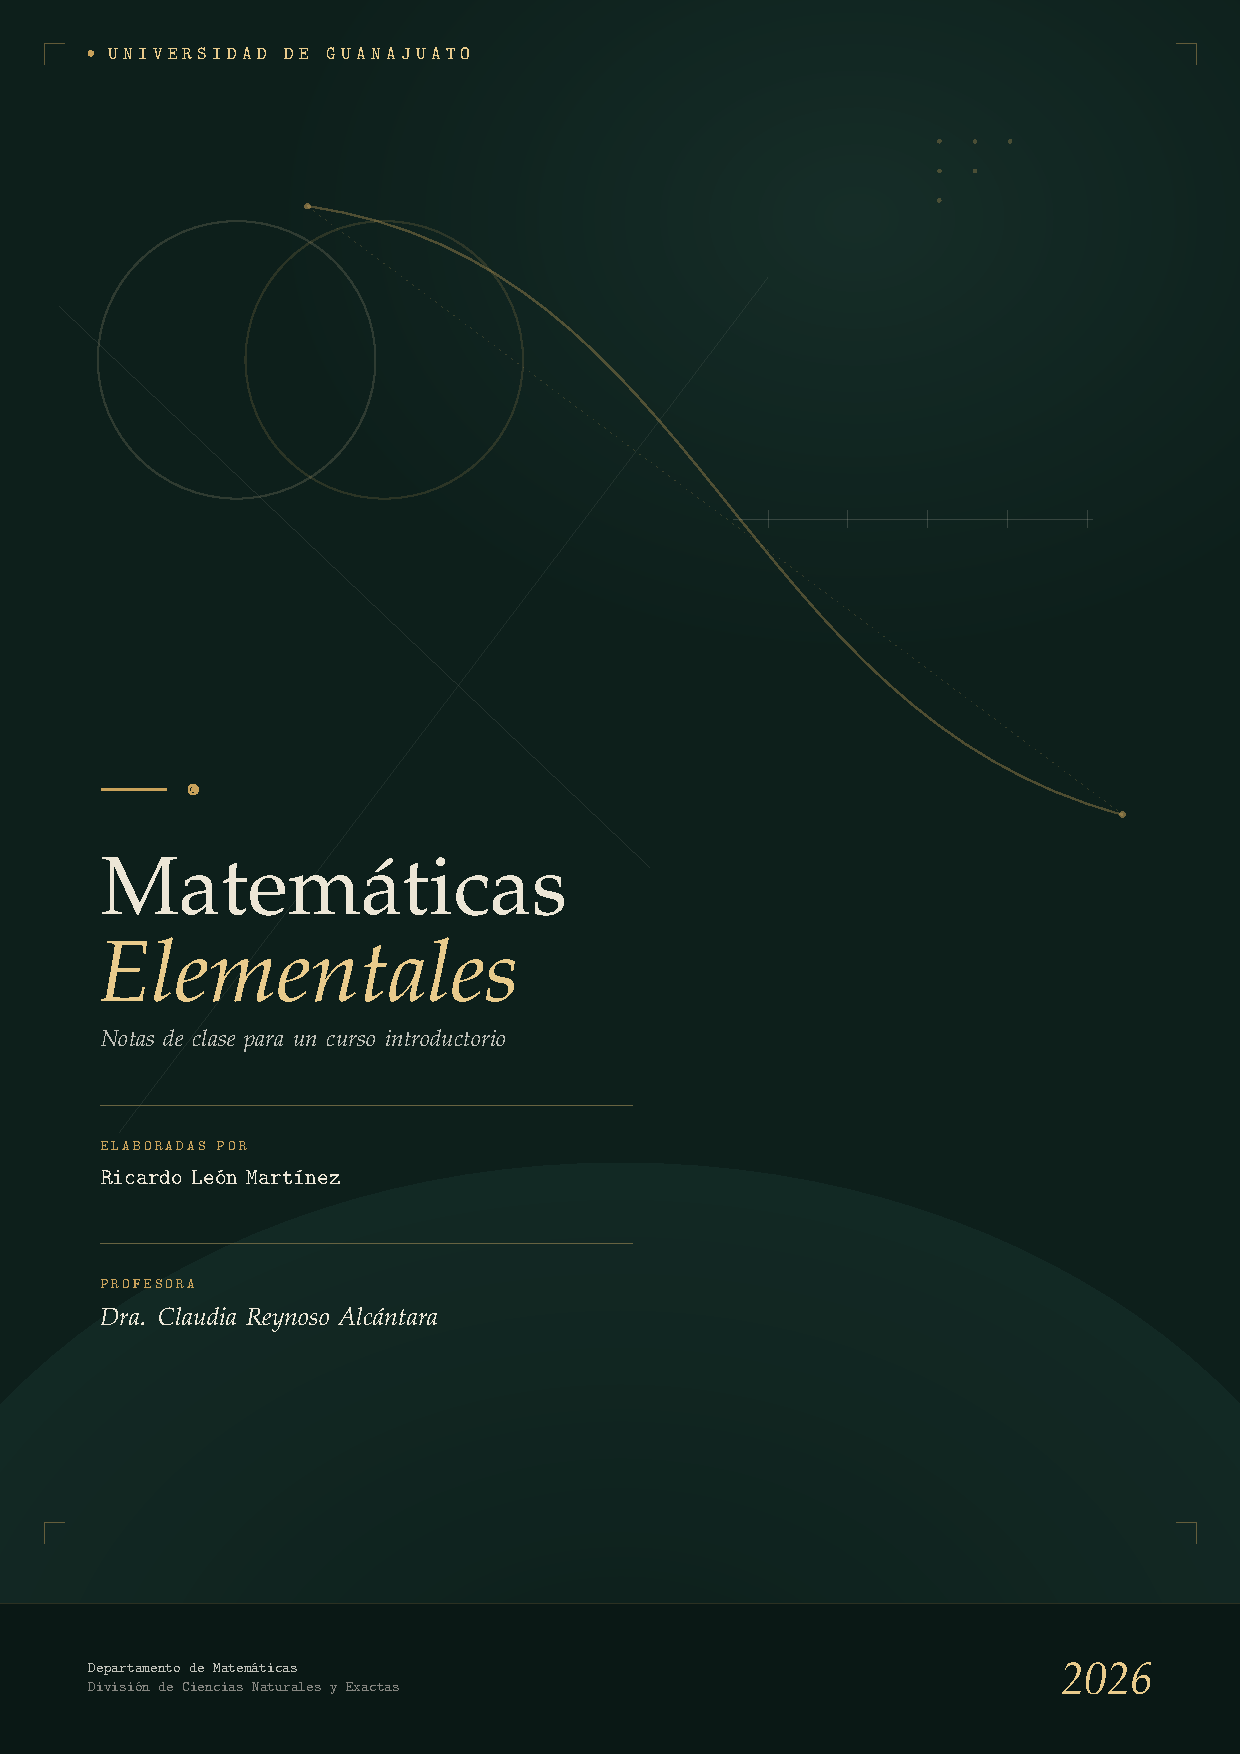
\includepdf[pages=1]{portada-matematicas-elementales.pdf}

    \begin{flushright}
      \thispagestyle{empty}

        \textbf{Ricardo}\\[0.3cm]
        \textit{A los tacos el paisa 2\\
        porque son unos rifados.\\
        A Román porque sufrió redactando\\
        estas notas.\\
        A Uicab por su libreta\\
        de lineal.\\
        Al grupo de todos ínfimos porque\\
        hacen más llevadera la universidad.\\
        Y a Sam, porque aunque no entienda\\
        del todo estas notas,\\
        siempre estuvo ahí.\\
        Y a Kaori, porque entre tareas, estrés\\
        y examenes, también estuvo ahí.}\\[1.2cm]
    \end{flushright}

    % ---------------- NOTA DE ERRORES ----------------

    \cleardoublepage
    \thispagestyle{empty}

    \begin{mdframed}[style=mdgreenbox]
        \begin{center}
        \small
        Estas notas fueron elaboradas con fines académicos.\\
        A pesar del cuidado puesto en su redacción,\\
        es posible que existan errores u omisiones.\\[0.3cm]

        Cualquier corrección, sugerencia o comentario será bienvenido
        en el correo: \\[0.3cm]

        ricardo.leon@cimat.mx
        \end{center}
    \end{mdframed}

    % -------------------------------------------------
    
    \setcounter{page}{1}
    \tableofcontents

    \chapter{Lógica proposicional}

    \section{Proposiciones y conectivos lógicos}

    Empezamos con el lenguaje que usaremos para enunciar y demostrar el resto de los resultados del curso: la lógica proposicional.

    \begin{definicion}[Proposición]
        Una \textbf{proposición} es una expresión que se puede calificar como verdadera o falsa, pero no ambas cosas a la vez.
    \end{definicion}

    A partir de proposiciones simples podemos construir proposiciones más complejas mediante los \textbf{conectivos lógicos}.

    \begin{definicion}[Negación]
        Sea $P$ una proposición. La \textbf{negación} de $P$, denotada por $\neg P$ (se lee ``no $P$''), es la proposición que satisface la siguiente tabla de verdad:
        \begin{equation*}
            \begin{array}{c|c}
                P & \neg P \\ \hline
                V & F      \\
                F & V
            \end{array}
        \end{equation*}
        donde $V$ significa verdadero y $F$ significa falso.
    \end{definicion}

    \begin{definicion}[Disyunción]
        Sean $P$ y $Q$ proposiciones. La \textbf{disyunción} de $P$ y $Q$, denotada por $P \vee Q$ (se lee ``$P$ o $Q$''), tiene la siguiente tabla de verdad:
        \begin{equation*}
            \begin{array}{cc|c}
                P & Q & P \vee Q \\ \hline
                V & V & V        \\
                V & F & V        \\
                F & V & V        \\
                F & F & F
            \end{array}
        \end{equation*}
    \end{definicion}

    \begin{definicion}[Conjunción]
        Sean $P$ y $Q$ proposiciones. La \textbf{conjunción} de $P$ y $Q$, denotada por $P \wedge Q$ (se lee ``$P$ y $Q$''), tiene la siguiente tabla de verdad:
        \begin{equation*}
            \begin{array}{cc|c}
                P & Q & P \wedge Q \\ \hline
                V & V & V          \\
                V & F & F          \\
                F & V & F          \\
                F & F & F
            \end{array}
        \end{equation*}
    \end{definicion}

    \begin{definicion}[Implicación]
        Sean $P$ y $Q$ proposiciones. La \textbf{implicación} de $P$ a $Q$, denotada por $P \Rightarrow Q$, se lee de cualquiera de las siguientes formas: ``$P$ implica $Q$'', ``si $P$ entonces $Q$'', ``de $P$ se sigue $Q$'', o ``$Q$ si $P$''. Su tabla de verdad es:
        \begin{equation*}
            \begin{array}{cc|c}
                P & Q & P \Rightarrow Q \\ \hline
                V & V & V               \\
                V & F & F               \\
                F & V & V               \\
                F & F & V
            \end{array}
        \end{equation*}
    \end{definicion}

    Notemos que $P \Rightarrow Q$ sólo es falsa cuando $P$ es verdadera y $Q$ es falsa; en cualquier otro caso es verdadera (en particular, una implicación con hipótesis falsa siempre es verdadera).

    \section{Cuantificadores}

    Los \textbf{cuantificadores} son símbolos que indican cuántos elementos de un conjunto satisfacen una proposición.

    \begin{definicion}[Cuantificadores]
        Sea $A$ un conjunto y $P$ una proposición sobre los elementos de $A$.
        \begin{itemize}
            \item El \textbf{cuantificador universal}, ``para todo'', se denota por $\forall$.
            \item El \textbf{cuantificador existencial}, ``existe'', se denota por $\exists$.
            \item El \textbf{cuantificador existencial único}, ``existe un único'', se denota por $\exists!$.
            \item El \textbf{cuantificador de no existencia}, ``no existe'', se denota por $\nexists$.
        \end{itemize}
    \end{definicion}

    \begin{ejemplo}
        \begin{equation*}
            \forall n \in \N,\ 2n \in \N
        \end{equation*}
        \begin{equation*}
            \exists n \in \N \text{ tal que } n+1=3
        \end{equation*}
        \begin{equation*}
            \exists! \, n \in \N \text{ tal que } n+1=2
        \end{equation*}
        \begin{equation*}
            \nexists\, n \in \N \text{ tal que } n+1=1
        \end{equation*}
    \end{ejemplo}

    Un aspecto importante de trabajar con cuantificadores es saber negar las proposiciones que los contienen.

    \begin{proposicion}[Negación de cuantificadores]
        Sea $A$ un conjunto y $P$ una proposición. Entonces:
        \begin{align*}
            \neg(\forall x\in A,\ x \text{ satisface } P)                    & \;\Longleftrightarrow\; \exists x\in A \text{ tal que } x \text{ no satisface } P,                    \\
            \neg(\exists x\in A \text{ tal que } x \text{ satisface } P)     & \;\Longleftrightarrow\; \forall x\in A,\ x \text{ no satisface } P,                                   \\
            \neg(\exists! \, x\in A \text{ tal que } x \text{ satisface } P) & \;\Longleftrightarrow\; \big(\exists\, x,y\in A,\ x\neq y,\ x \text{ y } y \text{ satisfacen } P\big) \\
                                                                             & \qquad \vee \big(\forall x\in A,\ x \text{ no satisface } P\big).
        \end{align*}
    \end{proposicion}

    En palabras: negar ``para todos'' produce ``existe uno que no''; negar ``existe uno'' produce ``ninguno lo satisface''; y negar ``existe exactamente uno'' produce ``hay al menos dos que lo satisfacen, o ninguno lo satisface''.

    \chapter{Tipos de demostración}

    Antes de continuar, conviene precisar los métodos de demostración que usaremos a lo largo del curso.

    \section{Demostración directa}

    Para probar $P\Rightarrow Q$, suponemos que se da $P$ y probamos que se da $Q$.

    \begin{ejemplo}
        \textbf{Demostración directa.}
        Si $n\in\N$ es par, entonces $n^2$ es par.

        \textbf{Demostración.} Sea $n\in\N$ tal que $n$ es par. Esto significa que existe $k\in\N$ tal que $n=2k$. Elevando al cuadrado esta igualdad obtenemos $n^2 = 2^2k^2 = 2(2k^2)$. Concluimos que $n^2$ es par.
    \end{ejemplo}

    \section{Demostraciones indirectas}

    \subsection{Demostración por contrapositiva}

    Para probar $P\Rightarrow Q$, basta probar la proposición equivalente $\neg Q \Rightarrow \neg P$.

    \begin{ejemplo}
        \textbf{Demostración por contrapositiva.}
        Si $n\in\N$ y $n^2$ es par, entonces $n$ es par.

        \textbf{Demostración.} Probamos la contrapositiva: si $n$ no es par, entonces $n^2$ no es par. Sea $n\in\N$. Supongamos que $n$ no es par (es impar); existe $k\in\N$ tal que $n=2k-1$, así que
        \begin{equation*}
            n^2-1 = (2k-1)^2-1 = 4k^2-4k = 2(2k^2-2k),
        \end{equation*}
        es decir, $2$ divide a $n^2-1 = (n+1)(n-1)$. Como $2$ es primo, $2$ divide a $n+1$ o a $n-1$; en cualquiera de los dos casos se concluye que $n$ es impar, y por lo tanto $n^2 = (n^2-1)+1$ es impar (no es par).
    \end{ejemplo}

    \subsection{Demostración por reducción al absurdo}

    Este método se basa en la equivalencia lógica
    \begin{equation*}
        \neg(P\Rightarrow Q) \;\Longleftrightarrow\; P\wedge\neg Q.
    \end{equation*}
    Es decir, para probar $P\Rightarrow Q$ podemos suponer $P\wedge\neg Q$ y llegar a una contradicción.

    \begin{ejemplo}
        \textbf{Demostración por reducción al absurdo.}
        $\sqrt{2}$ no es un número racional.

        \textbf{Demostración.} Supongamos, por contradicción, que $\sqrt{2}$ es racional. Entonces existen $p,q\in\N$ tales que
        \begin{equation*}
            \sqrt{2} = \frac{p}{q},
        \end{equation*}
        y, sin pérdida de generalidad, podemos suponer que $p$ y $q$ son primos relativos (es decir, no tienen factores comunes salvo $1$). Elevando al cuadrado, $2=p^2/q^2$, así que $p^2=2q^2$. Como $p^2$ es par, $p$ es par, así que existe $k\in\N$ tal que $p=2k$. Sustituyendo, $4k^2=2q^2$, es decir, $q^2=2k^2$, así que $q^2$ es par y, por lo tanto, $q$ también es par. Esto contradice que $p$ y $q$ sean primos relativos. Concluimos que $\sqrt{2}$ no es racional.
    \end{ejemplo}

    \section{Demostración por inducción matemática}

    \begin{proposicion}[Principio de inducción matemática]
        Sea $S\subset\N$ tal que $1\in S$, y tal que $n\in S$ implica $n+1\in S$. Entonces $S=\N$.
    \end{proposicion}

    Este principio se estudiará con más detalle en el Capítulo \ref{chap:induccion}, y será, de hecho, uno de los axiomas que definen a $\N$ (Capítulo \ref{chap:numeros}).

    \begin{ejemplo}
        \textbf{Demostración por inducción.}
        Para todo $n\in\N$,
        \begin{equation*}
            \sum_{i=1}^n i = \frac{n(n+1)}{2}.
        \end{equation*}

        \textbf{Demostración.} Sea $S = \left\{n\in\N : \sum_{i=1}^n i = \dfrac{n(n+1)}{2}\right\}$. Probaremos que $S=\N$.

        \emph{Base:} $\displaystyle\sum_{i=1}^1 i = 1 = \frac{1(1+1)}{2}$, así que $1\in S$.

        \emph{Paso inductivo:} Supongamos que $n\in S$, es decir, $\sum_{i=1}^n i = \dfrac{n(n+1)}{2}$. Entonces
        \begin{equation*}
            \sum_{i=1}^{n+1} i = \sum_{i=1}^n i + (n+1) = \frac{n(n+1)}{2}+(n+1) = \frac{n(n+1)+2(n+1)}{2} = \frac{(n+1)[(n+1)+1]}{2}.
        \end{equation*}
        Concluimos que $n+1\in S$. Por el principio de inducción, $S=\N$.
    \end{ejemplo}

    \chapter{Teoría de conjuntos}

    \section{Conjuntos, subconjuntos y operaciones básicas}

    Sea $A$ un conjunto. Diremos que $A \subset B$ si $\forall x\in A,\ x\in B$ (es decir, todo elemento de $A$ es también elemento de $B$). Diremos que $A=B$ si $A\subset B$ y $B\subset A$.

    \begin{definicion}[Conjunto vacío]
        Existe un conjunto, llamado \textbf{conjunto vacío} y denotado por $\emptyset$, tal que $\emptyset \subset A$ para todo conjunto $A$.
    \end{definicion}

    \begin{proposicion}
        El conjunto vacío es el único conjunto que está contenido en todo conjunto.
    \end{proposicion}

    \begin{proof}
        Ya sabemos que $\emptyset \subset A$ para todo conjunto $A$. Falta ver que ningún otro conjunto tiene esta propiedad. Supongamos que $X$ es un conjunto tal que $X\subset A$ para todo conjunto $A$; en particular, tomando $A=\emptyset$, tenemos $X\subset\emptyset$. Si $X$ tuviera un elemento $x$, entonces $x\in\emptyset$, lo cual es imposible. Por lo tanto $X$ no tiene elementos, es decir, $X=\emptyset$.
    \end{proof}

    En lo que sigue, $U$ denota un conjunto universal fijo del cual $A$, $B$, $C$, \dots\ son subconjuntos, y $P$, $Q$ denotan las proposiciones (o condiciones) que los definen.

    \begin{definicion}[Unión]
        El conjunto \textbf{unión} de $A$ y $B$ se define como
        \begin{equation*}
            A\cup B = \{x\in U : x\in A \vee x\in B\}.
        \end{equation*}
    \end{definicion}

    \begin{ejemplo}
        Si $A=\{x\in U : x \text{ satisface } P\}$ y $B=\{x\in U : x \text{ satisface } Q\}$, entonces
        \begin{equation*}
            A\cup B = \{x\in U : x \text{ satisface } P \vee Q\}.
        \end{equation*}
    \end{ejemplo}

    \begin{definicion}[Intersección]
        El conjunto \textbf{intersección} de $A$ y $B$ se define como
        \begin{equation*}
            A\cap B = \{x\in U : x\in A \wedge x\in B\}.
        \end{equation*}
    \end{definicion}

    Análogamente al caso de la unión, si $A$ y $B$ están definidos por las condiciones $P$ y $Q$, entonces $A\cap B = \{x\in U : x \text{ satisface } P\wedge Q\}$. Decimos que $A\subset B$ si para todo $x\in U$ que satisface $P$ se tiene que $x$ satisface $Q$.

    \begin{definicion}[Complemento]
        El conjunto \textbf{complemento} de $A$ (respecto a $U$) se define como
        \begin{equation*}
            A^c = \{x\in U : x\notin A\}.
        \end{equation*}
    \end{definicion}

    Si $A=\{x\in U : x \text{ satisface } P\}$, entonces $A^c = \{x\in U : x \text{ satisface } \neg P\}$.

    \begin{definicion}[Diferencia]
        El conjunto \textbf{diferencia} de $A$ menos $B$ se define como
        \begin{equation*}
            A\setminus B = \{x\in U : x\in A \wedge x\notin B\}.
        \end{equation*}
    \end{definicion}

    \section{Propiedades de las operaciones de conjuntos}

    \begin{teorema}[Propiedades básicas]
        Dados $A,B$ conjuntos, se tiene:
        \begin{enumerate}[label=(\arabic*)]
            \item $A\cup B = B\cup A$ \quad (pues $P\vee Q \Leftrightarrow Q\vee P$)
            \item $A\cap B = B\cap A$ \quad (pues $P\wedge Q \Leftrightarrow Q\wedge P$)
            \item $\emptyset^c = U$
            \item $U^c = \emptyset$
            \item $A\cap \emptyset = \emptyset$
            \item $A\cup \emptyset = A$
            \item $A\setminus B = A\cap B^c$
            \item $(A^c)^c = A$
            \item $A\cup A^c = U$
            \item $A\cap A^c = \emptyset$
        \end{enumerate}
    \end{teorema}

    \begin{proposicion}[Asociatividad de la unión]
        Sean $A,B,C$ conjuntos. Entonces $A\cup(B\cup C) = (A\cup B)\cup C$.
    \end{proposicion}

    \begin{proof}
        Por doble contención.

        ($\subset$) Sea $x\in A\cup(B\cup C)$; esto significa que $x\in A$ o $x\in(B\cup C)$. Si $x\in A$, entonces $x\in A\cup B$, y por lo tanto $x\in (A\cup B)\cup C$. Si $x\in B\cup C$, entonces $x\in B$ o $x\in C$. Si $x\in B$, entonces $x\in A\cup B$, así que $x\in(A\cup B)\cup C$; si $x\in C$, directamente $x\in(A\cup B)\cup C$. En cualquier caso, $x\in(A\cup B)\cup C$. Hemos probado que $A\cup(B\cup C) \subset (A\cup B)\cup C$.

        ($\supset$) La segunda contención es análoga.
    \end{proof}

    \begin{proposicion}[Leyes distributivas]
        Sean $A,B,C$ conjuntos. Entonces
        \begin{enumerate}[label=(\roman*)]
            \item $A\cap(B\cup C) = (A\cap B)\cup(A\cap C)$,
            \item $A\cup(B\cap C) = (A\cup B)\cap(A\cup C)$.
        \end{enumerate}
    \end{proposicion}

    \begin{proposicion}[Leyes de De Morgan]
        Sean $A,B$ conjuntos. Entonces
        \begin{enumerate}[label=(\roman*)]
            \item $(A\cup B)^c = A^c \cap B^c$,
            \item $(A\cap B)^c = A^c \cup B^c$.
        \end{enumerate}
    \end{proposicion}

    \begin{proof}
        Probamos (i). Si $A=\{x\in U : x \text{ satisface } P\}$ y $B=\{x\in U : x \text{ satisface } Q\}$, entonces
        \begin{equation*}
            A^c\cap B^c = \{x\in U : x \text{ satisface } \neg P\} \cap \{x\in U: x \text{ satisface } \neg Q\} = \{x\in U : x \text{ satisface } \neg P \wedge \neg Q\}.
        \end{equation*}
        Por otro lado, $(A\cup B)^c = \{x\in U : x \text{ satisface } \neg(P\vee Q)\}$. Basta entonces observar que las proposiciones $\neg P \wedge \neg Q$ y $\neg(P\vee Q)$ son lógicamente equivalentes (ambas son verdaderas exactamente cuando $P$ y $Q$ son ambas falsas), de donde se sigue que $A^c\cap B^c = (A\cup B)^c$. La demostración de (ii) es análoga.
    \end{proof}

    \section{El conjunto potencia y el producto cartesiano}

    Los axiomas anteriores sobre conjuntos forman parte de un sistema más amplio conocido como los \textbf{axiomas de Zermelo--Fraenkel con el axioma de elección} (ZFC). El siguiente axioma nos permite formar el conjunto de todos los subconjuntos de un conjunto dado.

    \noindent\textbf{Axioma (del conjunto potencia).} Si $A$ es un conjunto, entonces
    \begin{equation*}
        \mathcal{P}(A) = \{B : B \text{ es subconjunto de } A\}
    \end{equation*}
    es un conjunto, llamado el \textbf{conjunto potencia} de $A$.

    \begin{proposicion}
        Si $A$ es un conjunto finito con $n$ elementos ($n=0$ o $n\in\N$), entonces $\mathcal{P}(A)$ tiene $2^n$ elementos.
    \end{proposicion}

    \begin{proof}
        Por inducción sobre $n$. Si $n=0$, entonces $A=\emptyset$ y $\mathcal{P}(A)=\{\emptyset\}$ tiene $1=2^0$ elemento. Supongamos que la propiedad es válida para todo conjunto con $k$ elementos, y sea $A$ un conjunto con $k+1$ elementos. Fijemos $a\in A$ y escribamos $A' = A\setminus\{a\}$, que tiene $k$ elementos. Todo subconjunto de $A$ o bien no contiene a $a$ (y por lo tanto es subconjunto de $A'$), o bien contiene a $a$ (y se obtiene añadiendo $a$ a un subconjunto de $A'$). Así, $\mathcal{P}(A)$ tiene el doble de elementos que $\mathcal{P}(A')$, es decir, $2\cdot 2^k = 2^{k+1}$.
    \end{proof}

    \begin{definicion}[Producto cartesiano]
        Sean $A,B$ conjuntos. Definimos el \textbf{producto cartesiano} $A\times B$ como el conjunto
        \begin{equation*}
            A\times B = \{(a,b) : a\in A,\ b\in B\}.
        \end{equation*}
        Un elemento $(a,b)\in A\times B$ se llama \textbf{par ordenado}. Diremos que $(a,b)=(c,d)$ (ambos en $A\times B$) si $a=c$ y $b=d$.
    \end{definicion}

    \chapter{Relaciones y funciones}

    \section{Relaciones}

    \begin{definicion}[Relación]
        Sean $A,B$ conjuntos. Una \textbf{relación de $A$ en $B$} es un subconjunto $R\subset A\times B$; equivalentemente, es un elemento de $\mathcal{P}(A\times B)$.
    \end{definicion}

    \begin{ejemplo}
        Sean $A=\{1,2,3\}$, $B=\{5,6,7\}$. Consideremos
        \begin{equation*}
            R_1 = \{(n,m)\in A\times B : n+1=m\} = \emptyset, \qquad R_2 = \{(n,m)\in A\times B : n+2=m\} = \{(3,5)\}.
        \end{equation*}
    \end{ejemplo}

    \section{Composición de relaciones}

    \begin{definicion}[Composición de relaciones]
        Sean $R\subset A\times B$ y $S\subset B\times C$ relaciones. Definimos la \textbf{composición} $S\circ R$ como la relación de $A$ en $C$ dada por
        \begin{equation*}
            S\circ R = \{(a,c)\in A\times C : \exists\, b\in B \text{ tal que } (a,b)\in R \text{ y } (b,c)\in S\}.
        \end{equation*}
    \end{definicion}

    \begin{ejemplo}
        Sean $A=\{1,2\}$, $B=\{\alpha,\beta\}$, $C=\{e,\pi\}$, $R=\{(1,\alpha),(1,\beta)\}$ y $S=\{(\alpha,\pi),(\beta,e)\}$. Entonces
        \begin{equation*}
            S\circ R = \{(1,\pi),(1,e)\}.
        \end{equation*}
    \end{ejemplo}

    \begin{proposicion}[Asociatividad de la composición]
        Sean $A_1,A_2,A_3,A_4$ conjuntos y $R_1\subset A_1\times A_2$, $R_2\subset A_2\times A_3$, $R_3\subset A_3\times A_4$ relaciones. Entonces
        \begin{equation*}
            R_3\circ(R_2\circ R_1) = (R_3\circ R_2)\circ R_1.
        \end{equation*}
    \end{proposicion}

    \begin{proof}
        Ambos lados son relaciones de $A_1$ en $A_4$, es decir, subconjuntos de $A_1\times A_4$. Calculamos:
        \begin{align*}
            R_3\circ(R_2\circ R_1) &= \{(a_1,a_4)\in A_1\times A_4 : \exists\, a_2\in A_2,\ a_3\in A_3 \text{ tales que } \\
            &\qquad (a_1,a_2)\in R_1,\ (a_2,a_3)\in R_2,\ (a_3,a_4)\in R_3\},
        \end{align*}
        \begin{align*}
            (R_3\circ R_2)\circ R_1 &= \{(a_1,a_4)\in A_1\times A_4 : \exists\, a_2\in A_2,\ a_3\in A_3 \text{ tales que } \\
            &\qquad (a_1,a_2)\in R_1,\ (a_2,a_3)\in R_2,\ (a_3,a_4)\in R_3\}.
        \end{align*}
        Ambos conjuntos están descritos por exactamente la misma condición, así que son iguales.
    \end{proof}

    \section{Funciones}

    \begin{definicion}[Función]
        Sean $A,B$ conjuntos. Una \textbf{función} de $A$ en $B$ es una relación $f\subset A\times B$ tal que:
        \begin{enumerate}[label=(\arabic*)]
            \item El conjunto $D_f = \{a\in A : \exists\, b\in B \text{ tal que } (a,b)\in f\}$ es igual a $A$ (es decir, todo elemento de $A$ está relacionado con algún elemento de $B$).
            \item Si $(a,b_1),(a,b_2)\in f$, entonces $b_1=b_2$ (es decir, cada elemento de $A$ está relacionado con un único elemento de $B$).
        \end{enumerate}
    \end{definicion}

    Escribimos $f:A\to B$, $a\mapsto f(a)$, donde $f(a)$ denota al único elemento $b\in B$ tal que $(a,b)\in f$. Al conjunto $A$ le llamamos el \textbf{dominio} de $f$, y a $B$ el \textbf{codominio}. La \textbf{imagen} de $f$ es el conjunto
    \begin{equation*}
        \operatorname{Im}(f) = \{f(a)\in B : a\in A\}.
    \end{equation*}

    \begin{ejemplo}
        $f:\N\to\N$, $n\mapsto n+1$. El dominio y el codominio coinciden (ambos son $\N$), pero $\operatorname{Im}(f)=\N\setminus\{1\}$.
    \end{ejemplo}

    \begin{proposicion}
        Si $f_1:A_1\to A_2$ y $f_2:A_2\to A_3$ son funciones, entonces $f_2\circ f_1$ es una función de $A_1$ en $A_3$.
    \end{proposicion}

    \begin{proof}
        Sea $a_1\in A_1$. Como $(a_1,f_1(a_1))\in A_1\times A_2$ y $f_1(a_1)\in A_2$, tenemos $f_2(f_1(a_1))\in A_3$, así que $(a_1,f_2(f_1(a_1)))\in f_2\circ f_1$; esto muestra que $D_{f_2\circ f_1}=A_1$.

        Para la unicidad, sean $a_3,a_3'\in A_3$ tales que $(a_1,a_3),(a_1,a_3')\in f_2\circ f_1$. Entonces existen $a_2,a_2'\in A_2$ tales que $(a_1,a_2)\in f_1$, $(a_2,a_3)\in f_2$, $(a_1,a_2')\in f_1$, $(a_2',a_3')\in f_2$. Como $f_1$ es función, $a_2=a_2'$. Como $f_2$ es función y $(a_2,a_3),(a_2,a_3')\in f_2$ (usando $a_2=a_2'$), concluimos que $a_3=a_3'$.
    \end{proof}

    \begin{definicion}[Relación inversa]
        Sea $R\subset A\times B$ una relación. Definimos la \textbf{relación inversa} de $R$ como
        \begin{equation*}
            R^{-1} = \{(b,a)\in B\times A : (a,b)\in R\}.
        \end{equation*}
    \end{definicion}

    \begin{proposicion}
        Sean $R_1\subset A_1\times A_2$, $R_2\subset A_2\times A_3$ relaciones. Entonces $(R_2\circ R_1)^{-1} = R_1^{-1}\circ R_2^{-1}$.
    \end{proposicion}

    \begin{proof}
        Sea $(a_3,a_1)\in(R_2\circ R_1)^{-1}$; esto equivale a $(a_1,a_3)\in R_2\circ R_1$, es decir, a que exista $a_2\in A_2$ con $(a_1,a_2)\in R_1$ y $(a_2,a_3)\in R_2$. Esto equivale a que exista $a_2$ con $(a_3,a_2)\in R_2^{-1}$ y $(a_2,a_1)\in R_1^{-1}$, es decir, a que $(a_3,a_1)\in R_1^{-1}\circ R_2^{-1}$.
    \end{proof}

    \begin{definicion}[Función identidad]
        Sea $A$ un conjunto. La \textbf{función identidad} de $A$ es
        \begin{equation*}
            \operatorname{Id}_A : A\to A, \qquad a\mapsto a.
        \end{equation*}
    \end{definicion}

    \begin{definicion}[Función característica]
        Sean $A$ un conjunto y $B\subset A$. La \textbf{función característica} de $B$ es
        \begin{equation*}
            \chi_B : A \to \{0,1\}, \qquad a\mapsto \begin{cases} 1 & \text{si } a\in B, \\ 0 & \text{si } a\notin B. \end{cases}
        \end{equation*}
    \end{definicion}

    \begin{lema}
        Sean $A,B$ conjuntos y $f:A\to B$ una función. Entonces
        \begin{equation*}
            f\circ \operatorname{Id}_A = f, \qquad \operatorname{Id}_B \circ f = f.
        \end{equation*}
    \end{lema}

    \begin{proof}
        Para $a\in A$, $(f\circ\operatorname{Id}_A)(a) = f(\operatorname{Id}_A(a)) = f(a)$; como esto vale para todo $a\in A$, $f\circ\operatorname{Id}_A=f$. Análogamente, $(\operatorname{Id}_B\circ f)(a) = \operatorname{Id}_B(f(a)) = f(a)$ para todo $a\in A$, así que $\operatorname{Id}_B\circ f=f$.
    \end{proof}

    \section{Inyectividad, sobreyectividad y biyectividad}

    \begin{definicion}[Función inyectiva]
        Sea $f:A\to B$ una función. Diremos que $f$ es \textbf{inyectiva} si satisface lo siguiente:
        \begin{equation*}
            \text{si } f(a_1)=f(a_2), \text{ entonces } a_1=a_2.
        \end{equation*}
    \end{definicion}

    \begin{ejemplo}
        $f:\R\to\R$, $x\mapsto 2x$, es inyectiva: si $f(x_1)=f(x_2)$, entonces $2x_1=2x_2$, así que $x_1=x_2$.

        $g:\R\to\R$, $x\mapsto x^2$, no es inyectiva, pues $g(1)=g(-1)=1$ pero $1\neq -1$.

        La función piso $\lfloor\cdot\rfloor:\R\to\Z$, $x\mapsto\lfloor x\rfloor$ (el máximo entero menor o igual que $x$), no es inyectiva: $\lfloor \tfrac12\rfloor = \lfloor 0\rfloor = 0$.

        La función identidad $\operatorname{Id}_A:A\to A$ siempre es inyectiva.
    \end{ejemplo}

    \begin{definicion}[Función sobreyectiva]
        Sea $f:A\to B$ una función. Diremos que $f$ es \textbf{sobreyectiva} (o \textbf{sobre}) si para todo $b\in B$ existe $a\in A$ tal que $f(a)=b$; equivalentemente, si $\operatorname{Im}(f)=B$.
    \end{definicion}

    \begin{definicion}[Función biyectiva]
        Sea $f:A\to B$ una función. Diremos que $f$ es \textbf{biyectiva} si $f$ es inyectiva y sobreyectiva.
    \end{definicion}

    \begin{ejemplo}
        \textbf{Las biyecciones de un conjunto de 3 elementos.}
        Sea $A=\{1,2,3\}$. Hay exactamente $3!=6$ funciones biyectivas de $A$ en $A$: la identidad, tres transposiciones (que intercambian dos elementos y fijan el tercero), y dos permutaciones cíclicas.
        \begin{equation*}
            \operatorname{Id}_A:\ 1\mapsto1,\ 2\mapsto2,\ 3\mapsto3
        \end{equation*}
        \begin{equation*}
            \sigma_1:\ 1\mapsto2,\ 2\mapsto1,\ 3\mapsto3 \qquad
            \sigma_2:\ 1\mapsto1,\ 2\mapsto3,\ 3\mapsto2 \qquad
            \sigma_3:\ 1\mapsto3,\ 2\mapsto2,\ 3\mapsto1
        \end{equation*}
        \begin{equation*}
            \sigma_4:\ 1\mapsto2,\ 2\mapsto3,\ 3\mapsto1 \qquad
            \sigma_5:\ 1\mapsto3,\ 2\mapsto1,\ 3\mapsto2
        \end{equation*}
    \end{ejemplo}

    \section{Inversas de una función}

    \begin{definicion}[Inversa izquierda e inversa derecha]
        Sea $f:A\to B$ una función. Diremos que una función $g:B\to A$ es una \textbf{inversa izquierda} de $f$ si $g\circ f = \operatorname{Id}_A$, y que es una \textbf{inversa derecha} de $f$ si $f\circ g = \operatorname{Id}_B$.
    \end{definicion}

    \begin{ejemplo}
        Sean $f:\Z\to\Z$, $n\mapsto 2n$, y $g:\Z\to\Z$, $n\mapsto\lfloor n/2\rfloor$. Entonces
        \begin{equation*}
            (g\circ f)(n) = g(2n) = \left\lfloor \frac{2n}{2}\right\rfloor = \lfloor n\rfloor = n,
        \end{equation*}
        así que $g\circ f = \operatorname{Id}_{\Z}$, es decir, $g$ es una inversa izquierda de $f$.
    \end{ejemplo}

    \begin{teorema}
        Sea $f\colon A \to B$ una función. Entonces $f$ es inyectiva si y sólo si tiene inversa izquierda.
    \end{teorema}
    \begin{proof}
        Supongamos primero que $f$ tiene una inversa izquierda $g:B\to A$, es decir, $g\circ f=\operatorname{Id}_A$. Si $a_1,a_2\in A$ satisfacen $f(a_1)=f(a_2)$, aplicando $g$ a ambos lados obtenemos
        \begin{equation*}
            a_1 = \operatorname{Id}_A(a_1) = g(f(a_1)) = g(f(a_2)) = \operatorname{Id}_A(a_2) = a_2,
        \end{equation*}
        así que $f$ es inyectiva.

        Recíprocamente, supongamos que $f$ es inyectiva. Definimos $g:B\to A$ por
        \begin{equation*}
            g(b) = \begin{cases} a & \text{si } b=f(a) \text{ para algún } a\in A, \\ \text{(elección arbitraria en $A$)} & \text{si } b\notin\operatorname{Im}(f). \end{cases}
        \end{equation*}
        Esto está bien definido: si $b\in\operatorname{Im}(f)$, como $f$ es inyectiva existe un único $a\in A$ tal que $f(a)=b$. Para $a\in A$, $(g\circ f)(a) = g(f(a)) = a$, pues $f(a)\in\operatorname{Im}(f)$ proviene precisamente de $a$. Así, $g\circ f=\operatorname{Id}_A$.
    \end{proof}

    Cuando $f$ tiene inversa izquierda, ésta no siempre es única.

    \begin{ejemplo}
        \textbf{No unicidad de la inversa izquierda.}
        Sean $A=\{1,2\}$, $B=\{a,b,c\}$, y $f:A\to B$ dada por $f(1)=a$, $f(2)=b$. Definamos $g_1,g_2:B\to A$ por
        \begin{equation*}
            g_1(a)=1,\ g_1(b)=2,\ g_1(c)=1, \qquad g_2(a)=1,\ g_2(b)=2,\ g_2(c)=2.
        \end{equation*}
        Es fácil verificar que $g_1\circ f = g_2\circ f = \operatorname{Id}_A$, así que $f$ tiene (al menos) dos inversas izquierdas distintas. Notemos que $f$ no es sobreyectiva.
    \end{ejemplo}

    \begin{teorema}
        Sea $f\colon A \to B$ una función. Entonces $f$ es sobre si y sólo si $f$ tiene inversa derecha.
    \end{teorema}
    \begin{proof}
        Supongamos que $f\colon A \to B$ es sobre. Queremos construir una función $g\colon B \to A$ tal que $f \circ g = \operatorname{Id}_B$. Como $f$ es sobre, $\operatorname{Im}(f) = \{f(a) : a \in A\} = B$. Luego, para cada $b \in B$ existe $a \in A$ tal que $f(a) = b$; tomamos uno de tales $a$ y definimos $g(b) = a$ (esta elección simultánea para todo $b\in B$ está garantizada por el axioma de elección). Construida $g\colon B \to A$ de esta forma, para todo $b \in B$ se tiene
        \begin{equation*}
            (f \circ g)(b) = f(g(b)) = f(a) = b,
        \end{equation*}
        por lo tanto $f \circ g = \operatorname{Id}_B$.

        Supongamos ahora que existe $g\colon B \to A$ inversa derecha de $f$, es decir,
        \begin{equation*}
            f \circ g = \operatorname{Id}_B.
        \end{equation*}
        Sea $b \in B$; tenemos que probar que existe $a \in A$ tal que $f(a) = b$. Sea $g(b) \in A$; entonces
        \begin{equation*}
            f(g(b)) = b,
        \end{equation*}
        así que existe $a = g(b) \in A$ tal que $f(a) = f(g(b)) = b$. Por lo tanto $f\colon A \to B$ es sobre.
    \end{proof}

    \begin{proposicion}
        Si la función $f\colon A \to B$ tiene una inversa izquierda $g\colon B \to A$ y una inversa derecha $h\colon B \to A$, entonces $g = h$.
    \end{proposicion}
    \begin{proof}
        Por hipótesis $g \circ f = \operatorname{Id}_A$ y $f \circ h = \operatorname{Id}_B$, así que
        \begin{equation*}
            g = g \circ \operatorname{Id}_B = g \circ (f \circ h) = (g \circ f) \circ h = \operatorname{Id}_A \circ h = h.
        \end{equation*}
    \end{proof}

    \begin{definicion}
        Una función $f\colon A \to B$ se dice \textbf{invertible} si tiene inversa izquierda e inversa derecha. (Por la proposición anterior, éstas coinciden y son únicas.)
    \end{definicion}

    \begin{corolario}
        Sea $f\colon A \to B$ función. Entonces $f$ es invertible si y sólo si $f$ es biyectiva. En este caso existe una única $g\colon B \to A$ tal que
        \begin{equation*}
            f \circ g = \operatorname{Id}_B, \qquad g \circ f = \operatorname{Id}_A.
        \end{equation*}
    \end{corolario}

    \section{Conjuntos numerables}

    \begin{definicion}
        Un conjunto $A$ se dice \textbf{numerable} si existe una función biyectiva
        \begin{equation*}
            f \colon \N \to A.
        \end{equation*}
    \end{definicion}

    \begin{proposicion}
        $\Z$ es un conjunto numerable.
    \end{proposicion}

    \section{Imagen inversa}

    \begin{definicion}
        Sea $f\colon A \to B$ una función y sea $C \subset B$. La \textbf{imagen inversa} (o preimagen) de $C$ bajo $f$ se define como el conjunto
        \begin{equation*}
            f^{-1}(C) = \{a \in A : f(a) \in C\} \subset A.
        \end{equation*}
    \end{definicion}

    \begin{ejemplo}
        Sea $f\colon \R \to \R$, $x \mapsto x^2$, y sea $C = \{1\}$. Entonces
        \begin{equation*}
            f^{-1}(C) = \{-1,1\}.
        \end{equation*}
        Además,
        \begin{align*}
            f^{-1}([1,4]) &= \{x \in \R : x^2 \in [1,4]\} \\
            &= \{x \in \R : 1 \le x^2 \le 4\} \\
            &= [-2,-1] \cup [1,2].
        \end{align*}
    \end{ejemplo}

    \begin{ejemplo}
        Sea $f\colon \R \to \R$, $x \mapsto 2x+1$. Entonces
        \begin{equation*}
            f^{-1}([3,7]) = \{x \in \R : 2x+1 \in [3,7]\}.
        \end{equation*}
        Como
        \begin{equation*}
            3 \le 2x+1 \le 7 \; \Longleftrightarrow \; 2 \le 2x \le 6 \; \Longleftrightarrow \; 1 \le x \le 3,
        \end{equation*}
        se tiene que $f^{-1}([3,7]) = [1,3]$.
    \end{ejemplo}

    \begin{proposicion}
        Sea $f\colon A \to B$ una función. Entonces
        \begin{enumerate}
            \item $f^{-1}(\emptyset) = \emptyset$.
            \item $f^{-1}(B) = A$.
            \item Si $C, D \subset B$, entonces $f^{-1}(C \cup D) = f^{-1}(C) \cup f^{-1}(D)$.
            \item Si $C, D \subset B$, entonces $f^{-1}(C \cap D) = f^{-1}(C) \cap f^{-1}(D)$.
        \end{enumerate}
    \end{proposicion}
    \begin{proof}[Demostración (sólo de (3))]
        Tenemos
        \begin{equation*}
            f^{-1}(C \cup D) = \{a \in A : f(a) \in C \cup D\}
        \end{equation*}
        y
        \begin{equation*}
            f^{-1}(C) \cup f^{-1}(D) = \{a \in A : f(a) \in C\} \cup \{a \in A : f(a) \in D\}.
        \end{equation*}
        Si $a \in f^{-1}(C \cup D)$, entonces $f(a) \in C$ o $f(a) \in D$, así que $a \in f^{-1}(C) \cup f^{-1}(D)$. Recíprocamente, si $a \in f^{-1}(C) \cup f^{-1}(D)$, entonces $f(a) \in C$ o $f(a) \in D$, es decir, $f(a) \in C \cup D$, por lo que $a \in f^{-1}(C \cup D)$. Por lo tanto $f^{-1}(C \cup D) = f^{-1}(C) \cup f^{-1}(D)$.
    \end{proof}

    \chapter{Inducción matemática}
    \label{chap:induccion}

    En el Capítulo 2 introdujimos el principio de inducción matemática como método de demostración. En este capítulo lo estudiamos con más detalle: damos una versión más general (con base en cualquier $n_0\in\N$) y el principio de inducción fuerte.

    \section{El principio de inducción}

    \begin{proposicion}[Principio de inducción, versión general]
        Sea $n_0\in\N$ y sea $S \subset \{n\in\N : n\ge n_0\}$ tal que:
        \begin{enumerate}[label=(\alph*)]
            \item $n_0 \in S$,
            \item para todo $n\ge n_0$, si $n\in S$ entonces $n+1\in S$.
        \end{enumerate}
        Entonces $S=\{n\in\N : n\ge n_0\}$.
    \end{proposicion}

    \begin{ejemplo}
        Para todo $n\in\N$ con $n\ge 5$, $2^n > n^2$.

        \textbf{Demostración.} Sea $S=\{n\in\N : n\ge 5,\ 2^n>n^2\}$. Como $2^5=32>25=5^2$, se tiene $5\in S$. Supongamos que $n\ge 5$ y $n\in S$, es decir $2^n>n^2$. Como $n\ge5$, se tiene $n^2>2n+1$, así que
        \begin{equation*}
            2^{n+1} = 2\cdot 2^n > 2n^2 = n^2+n^2 > n^2+2n+1 = (n+1)^2.
        \end{equation*}
        Por tanto $n+1\in S$, y por el principio de inducción (con $n_0=5$), $S=\{n\in\N : n\ge5\}$.
    \end{ejemplo}

    \section{Inducción fuerte}

    \begin{proposicion}[Principio de inducción fuerte]
        Sea $S\subset\N$ tal que:
        \begin{enumerate}[label=(\alph*)]
            \item $1\in S$,
            \item para todo $n\in\N$, si $\{1,2,\dots,n\}\subset S$, entonces $n+1\in S$.
        \end{enumerate}
        Entonces $S=\N$.
    \end{proposicion}

    \begin{proof}
        Sea $T=\{n\in\N : \{1,\dots,n\}\subset S\}$. Probaremos que $T=\N$ usando el principio de inducción (ordinario).

        \emph{Base.} Como $1\in S$ por (a), se tiene $\{1\}\subset S$, así que $1\in T$.

        \emph{Paso inductivo.} Supongamos que $n\in T$, es decir, $\{1,\dots,n\}\subset S$. Por (b), $n+1\in S$; por lo tanto $\{1,\dots,n+1\} = \{1,\dots,n\}\cup\{n+1\}\subset S$, es decir, $n+1\in T$.

        Por el principio de inducción, $T=\N$. Como $n\in\{1,\dots,n\}\subset S$ para todo $n\in T$, concluimos que $S=\N$.
    \end{proof}

    \chapter{Relaciones de equivalencia}

    \section{Propiedades de una relación}

    Sea $A$ un conjunto y $R\subset A\times A$ una relación de $A$ en $A$.

    \begin{definicion}[Propiedades de una relación]
        Diremos que $R$ es:
        \begin{enumerate}[label=(\alph*)]
            \item \textbf{Reflexiva}, si para todo $a\in A$ se tiene $(a,a)\in R$.
            \item \textbf{Simétrica}, si siempre que $(a_1,a_2)\in R$, se tiene que $(a_2,a_1)\in R$.
            \item \textbf{Transitiva}, si siempre que $(a_1,a_2)\in R$ y $(a_2,a_3)\in R$, se tiene que $(a_1,a_3)\in R$.
        \end{enumerate}
    \end{definicion}

    \begin{ejemplo}
        Sea $A=\N$ y $R_1 = \{(n,m)\in A\times A : n-m \text{ es par}\}$.

        $R_1$ es reflexiva: dado $n\in A$, $n-n=0$ es par, así que $(n,n)\in R_1$.

        $R_1$ es simétrica: si $(n,m)\in R_1$, existe $k\in\Z$ tal que $n-m=2k$; multiplicando por $-1$, $m-n=2(-k)$, así que $(m,n)\in R_1$.

        $R_1$ es transitiva: si $(n,m),(m,l)\in R_1$, existen $m_1,m_2\in\Z$ tales que $n-m=2m_1$ y $m-l=2m_2$; sumando, $n-l = 2(m_1+m_2)$, así que $(n,l)\in R_1$.

        Consideremos ahora $R_2 = \{(n,m)\in A\times A : n^2=m\}$. $R_2$ no es reflexiva, pues $(2,2)\notin R_2$ (ya que $2^2=4\neq 2$). Tampoco es simétrica, pues $(2,4)\in R_2$ pero $(4,2)\notin R_2$ (ya que $4^2=16\neq 2$). Y tampoco es transitiva, pues $(2,4),(4,16)\in R_2$ pero $(2,16)\notin R_2$.
    \end{ejemplo}

    Notemos que si $A=\emptyset$, la relación $R=\emptyset$ es reflexiva y simétrica de manera trivial. Si $A\neq\emptyset$, la relación $R=A\times A$ (donde todo par está relacionado) también es reflexiva y simétrica.

    \section{Relaciones de equivalencia}

    \begin{definicion}[Relación de equivalencia]
        Una relación $R\subset A\times A$ que es reflexiva, simétrica y transitiva se llama \textbf{relación de equivalencia} en $A$.
    \end{definicion}

    \begin{ejemplo}
        \textbf{Congruencia módulo $n$.}
        Sea $n\in\N$. Definimos en $\Z$ la relación
        \begin{equation*}
            R = \{(k,j)\in\Z\times\Z : k-j \text{ es múltiplo de } n\}.
        \end{equation*}
        Probemos que $R$ es una relación de equivalencia.

        \textbf{Reflexividad.} Sea $k\in\Z$. Como $k-k=0\cdot n$, se tiene $(k,k)\in R$.

        \textbf{Simetría.} Sea $(k,j)\in R$; existe $m\in\Z$ tal que $k-j=mn$. Multiplicando por $-1$, $j-k=(-m)n$, así que $(j,k)\in R$.

        \textbf{Transitividad.} Supongamos que $(k,j),(j,l)\in R$; existen $m_1,m_2\in\Z$ tales que $k-j=m_1n$ y $j-l=m_2n$. Sumando ambas ecuaciones, $k-l = m_1n+m_2n=(m_1+m_2)n$, así que $(k,l)\in R$.

        Concluimos que $R$ es una relación de equivalencia en $\Z$, conocida como la \textbf{congruencia módulo $n$}.
    \end{ejemplo}

    \section{Clases de equivalencia}

    \begin{definicion}[Clase de equivalencia]
        Sea $A$ un conjunto y $R\subset A\times A$ una relación de equivalencia. Dado $a\in A$, definimos la \textbf{clase de equivalencia} de $a$ respecto a $R$ como el conjunto
        \begin{equation*}
            [a]_R = \{b\in A : (a,b)\in R\}.
        \end{equation*}
    \end{definicion}

    Como $R$ es reflexiva, $\forall a\in A$, $a\in[a]_R$ (pues $(a,a)\in R$); en particular, ninguna clase de equivalencia es vacía.

    \begin{proposicion}
        Sea $A$ un conjunto y $R$ una relación de equivalencia en $A$. Entonces las clases de equivalencia satisfacen:
        \begin{enumerate}[label=(\arabic*)]
            \item Dados $a_1,a_2\in A$, o bien $[a_1]_R\cap[a_2]_R=\emptyset$, o bien $[a_1]_R=[a_2]_R$.
            \item $A = \displaystyle\bigcup_{a\in A}[a]_R$.
        \end{enumerate}
    \end{proposicion}

    \begin{proof}
        (1) Sean $a_1,a_2\in A$ y supongamos que $[a_1]_R\cap[a_2]_R\neq\emptyset$; probaremos que $[a_1]_R=[a_2]_R$. Existe $b\in[a_1]_R\cap[a_2]_R$, es decir, $(a_1,b),(a_2,b)\in R$. Como $R$ es simétrica, $(b,a_1),(b,a_2)\in R$. Como $R$ es transitiva, de $(a_1,b),(b,a_2)\in R$ concluimos $(a_1,a_2)\in R$.

        Sea $c\in[a_2]_R$, es decir, $(a_2,c)\in R$; como $(a_1,a_2)\in R$, por transitividad $(a_1,c)\in R$, así que $c\in[a_1]_R$. Hemos probado que $[a_2]_R\subset[a_1]_R$; la contención $[a_1]_R\subset[a_2]_R$ es análoga. Concluimos que $[a_1]_R=[a_2]_R$.

        (2) Para todo $a\in A$, $[a]_R\subset A$, así que $\bigcup_{a\in A}[a]_R \subset A$. Recíprocamente, sea $a_1\in A$; por la reflexividad, $a_1\in[a_1]_R$, así que $a_1\in\bigcup_{a\in A}[a]_R$. Concluimos que $A=\bigcup_{a\in A}[a]_R$.
    \end{proof}

    El resultado anterior dice que las clases de equivalencia de una relación de equivalencia en $A$ \textbf{particionan} a $A$: son disjuntas dos a dos, y su unión es todo $A$.

    \chapter{Introducción a la construcción de las estructuras numéricas}
    \label{chap:numeros}
    \chaptermark{Estructuras numéricas}

    En este capítulo iniciamos la construcción de las estructuras numéricas del curso. Empezamos por los números naturales $\N$: los tomamos como un objeto dado axiomáticamente (los axiomas de Peano) y, a partir de ellos, definimos sus operaciones y demostramos sus propiedades. Las demás estructuras numéricas (los enteros, los racionales, \dots) se construirán en secciones posteriores de este capítulo, a partir de $\N$, conforme se vean en el curso.

    \section{Los números naturales}

    \subsection{Axiomas de Peano}

    \medskip
    \noindent\textbf{Axioma de Peano.} Existe un conjunto $\N$ con las siguientes propiedades:
    \begin{enumerate}
        \item[(1)] $\N$ contiene un elemento llamado uno, denotado por $1$.
        \item[(2)] Existe una función inyectiva
        \begin{equation*}
            \sigma \colon \N \to \N, \qquad n \mapsto n+1 := \sigma(n).
        \end{equation*}
        A la imagen $\sigma(n)$ se le llama el \textbf{sucesor} de $n$.
        \item[(3)] No existe $n \in \N$ tal que $\sigma(n) = 1$ (es decir, para todo $n \in \N$, $\sigma(n) \ne 1$). En particular,
        \begin{equation*}
            \operatorname{Im}(\sigma) = \{\sigma(n) : n \in \N\} = \N \setminus \{1\}.
        \end{equation*}
        \item[(4)] (Principio de inducción) Si $S \subseteq \N$ es tal que
        \begin{enumerate}
            \item[(a)] $1 \in S$,
            \item[(b)] si $n \in S$, entonces $\sigma(n) \in S$,
        \end{enumerate}
        entonces $S = \N$.
    \end{enumerate}
    Este conjunto se llama el \textbf{conjunto de los números naturales}. El apartado (4) es precisamente el principio de inducción estudiado en el Capítulo \ref{chap:induccion}.
    \medskip

    \subsection{La suma}

    \begin{definicion}[Suma]
        Definimos una operación binaria en $\N$, llamada \textbf{suma} y denotada por $+$, de la siguiente manera:
        \begin{equation*}
            +\colon \N \times \N \to \N,
        \end{equation*}
        \begin{enumerate}
            \item[(1)] si $n \in \N$, $n+1 := \sigma(n)$;
            \item[(2)] si $n,m \in \N$, $n + \sigma(m) := \sigma(n+m)$.
        \end{enumerate}
    \end{definicion}

    \begin{proposicion}
        Dados $n,m,l \in \N$ se tiene que la suma es asociativa, es decir,
        \begin{equation*}
            n + (m+l) = (n+m)+l.
        \end{equation*}
    \end{proposicion}
    \begin{proof}
        Definimos
        \begin{equation*}
            S = \{l \in \N : \forall n,m \in \N, \; (n+m)+l = n+(m+l)\}.
        \end{equation*}
        Tenemos que probar, por inducción, que $S = \N$.

        Sean $n,m \in \N$. Entonces
        \begin{equation*}
            (n+m)+1 = \sigma(n+m) = n + \sigma(m) = n+(m+1).
        \end{equation*}
        Así que $1 \in S$.

        Supongamos que $l \in S$; queremos probar que $\sigma(l) \in S$. Sean $n,m \in \N$; entonces
        \begin{align*}
            n + (m + \sigma(l)) &= n + \sigma(m+l) \\
            &= \sigma(n+(m+l)) \\
            &= \sigma((n+m)+l) \\
            &= (n+m) + \sigma(l).
        \end{align*}
        Así que $\sigma(l) \in S$. Por tanto $S = \N$.
    \end{proof}

    \begin{ejemplo}
        Consideremos la afirmación ``para todo $n \in \N$, $n^2+n+1$ es par'' y sea
        \begin{equation*}
            S = \{n \in \N : n^2+n+1 \text{ es par}\}.
        \end{equation*}
        Si $n \in S$, entonces $n^2+n+1 = 2k$ para algún $k \in \N$, y
        \begin{equation*}
            (n+1)^2+(n+1)+1 = n^2+n+1+2n+2 = 2(k+n+1),
        \end{equation*}
        así que si $n \in S$ entonces $n+1 \in S$. Sin embargo $1^2+1+1=3$ no es par, es decir $1 \notin S$, de modo que $S \ne \N$: la afirmación es falsa a pesar de que se cumple el paso inductivo. Esto muestra que verificar únicamente el paso inductivo, sin la base, no basta para aplicar el principio de inducción.
    \end{ejemplo}

    \begin{proposicion}
        La suma en $\N$ es conmutativa, es decir, para todo $n,m \in \N$ se tiene que
        \begin{equation*}
            n+m = m+n.
        \end{equation*}
    \end{proposicion}
    \begin{proof}
        Sea
        \begin{equation*}
            S = \{n \in \N : \forall m \in \N, \; n+m=m+n\}.
        \end{equation*}
        Para probar que $1 \in S$, definimos primero
        \begin{equation*}
            T = \{n \in \N : n+1 = 1+n\}.
        \end{equation*}
        Tenemos que $1 \in T$ porque $1+1=1+1$. Supongamos que $n \in T$; queremos probar que $\sigma(n) \in T$:
        \begin{equation*}
            1+\sigma(n) = \sigma(1+n) = \sigma(n+1) = \sigma(\sigma(n)) = \sigma(n)+1.
        \end{equation*}
        Por tanto $T = \N$, es decir $1+n=n+1$ para todo $n \in \N$; en particular $1 \in S$.

        Supongamos ahora que $n \in S$; sea $m \in \N$:
        \begin{align*}
            m+\sigma(n) &= m+(n+1) = (m+n)+1 = (n+m)+1 \\
            &= 1+(n+m) = (1+n)+m = (n+1)+m = \sigma(n)+m.
        \end{align*}
        Así que $\sigma(n) \in S$. Por tanto $S = \N$.
    \end{proof}

    \begin{proposicion}
        Sean $n,m,l \in \N$ tales que $n+l = m+l$. Entonces $n=m$.
    \end{proposicion}
    \begin{proof}
        Sea
        \begin{equation*}
            S = \{l \in \N : \text{si } n+l=m+l \text{ con } n,m \in \N, \text{ entonces } n=m\}.
        \end{equation*}
        Vamos a probar que $1 \in S$. Supongamos que
        \begin{equation*}
            n+1=m+1,
        \end{equation*}
        es decir $\sigma(n)=\sigma(m)$. Por el axioma (3), $\sigma$ es inyectiva, por lo tanto $n=m$. Así que $1 \in S$.

        Supongamos que $l \in S$ y que
        \begin{equation*}
            n+\sigma(l) = m+\sigma(l),
        \end{equation*}
        donde $n,m \in \N$. Tenemos que probar que $n=m$. Como $n+\sigma(l)=\sigma(n+l)$ y $m+\sigma(l)=\sigma(m+l)$, se tiene $\sigma(n+l)=\sigma(m+l)$; por la inyectividad de $\sigma$, $n+l=m+l$, y por hipótesis de inducción $n=m$. Así que $\sigma(l) \in S$. Por lo tanto $S=\N$.
    \end{proof}

    \subsection{El producto}

    \begin{definicion}[Producto]
        Definimos una operación binaria en $\N$, llamada \textbf{producto} y denotada por $\cdot$, mediante la regla
        \begin{equation*}
            \cdot \colon \N \times \N \to \N,
        \end{equation*}
        \begin{enumerate}
            \item[(1)] $\forall n \in \N$, $n \cdot 1 = n$;
            \item[(2)] $\forall n,m \in \N$, $n \cdot \sigma(m) = n\cdot m + n$.
        \end{enumerate}
    \end{definicion}

    \begin{proposicion}
        Para todo $n \in \N$,
        \begin{equation*}
            1 \cdot n = n.
        \end{equation*}
    \end{proposicion}
    \begin{proof}
        Sea
        \begin{equation*}
            S = \{n \in \N : 1 \cdot n = n\}.
        \end{equation*}
        $1 \in S$ porque $1 \cdot 1 = 1$. Supongamos que $n \in S$:
        \begin{equation*}
            1 \cdot \sigma(n) = 1 \cdot n + 1 = n+1 = \sigma(n).
        \end{equation*}
        Por tanto $\sigma(n) \in S$, así que $S = \N$.
    \end{proof}

    \begin{proposicion}
        Para todo $n,m,l \in \N$:
        \begin{enumerate}[label=(\arabic*)]
            \item El producto es conmutativo, es decir, $n \cdot m = m \cdot n$.
            \item El producto es asociativo, es decir, $(n \cdot m) \cdot l = n \cdot (m \cdot l)$.
        \end{enumerate}
    \end{proposicion}

    \begin{proposicion}
        Sean $n,m,l \in \N$. Entonces
        \begin{equation*}
            n \cdot (m+l) = n \cdot m + n \cdot l.
        \end{equation*}
    \end{proposicion}
    \begin{proof}
        Sea
        \begin{equation*}
            S = \{l \in \N : \forall n,m \in \N, \; n\cdot(m+l) = n\cdot m+n\cdot l\}.
        \end{equation*}
        Vamos a probar que $1 \in S$. Sean $n,m \in \N$:
        \begin{equation*}
            n\cdot(m+1) = n \cdot \sigma(m) = n\cdot m+n = n \cdot m+n\cdot 1.
        \end{equation*}
        Así que $1 \in S$. Supongamos que $l \in S$; sean $n,m \in \N$:
        \begin{align*}
            n\cdot(m+\sigma(l)) &= n\cdot \sigma(m+l) = n\cdot(m+l)+n \\
            &= (n\cdot m+n\cdot l)+n = n\cdot m+(n\cdot l+n) = n\cdot m+n\cdot \sigma(l).
        \end{align*}
        Así que $\sigma(l) \in S$. Por tanto $S=\N$.
    \end{proof}

    \subsection{Orden}

    \begin{definicion}
        Sean $n,m \in \N$. Diremos que $n$ es \textbf{menor} que $m$, y escribiremos $n < m$, si existe $k \in \N$ tal que
        \begin{equation*}
            n+k=m.
        \end{equation*}
        Escribiremos $n \le m$ si $n<m$ o $n=m$. Escribiremos $n>m$ si $m<n$, y $n\ge m$ si $m\le n$.
    \end{definicion}

    \begin{lema}[Transitividad del orden]
        \label{lem:orden-transitivo}
        Sean $n,m,l\in\N$ tales que $n<m$ y $m<l$. Entonces $n<l$.
    \end{lema}
    \begin{proof}
        Como $n<m$ y $m<l$, existen $k_1,k_2\in\N$ tales que $n+k_1=m$ y $m+k_2=l$. Entonces
        \begin{equation*}
            l = m+k_2 = (n+k_1)+k_2 = n+(k_1+k_2),
        \end{equation*}
        así que $n<l$.
    \end{proof}

    \begin{lema}
        \label{lem:sucesor-distinto}
        Para todo $m\in\N$, $m\neq\sigma(m)$.
    \end{lema}
    \begin{proof}
        Sea $S=\{m\in\N : m\neq\sigma(m)\}$. Si $1=\sigma(1)$, esto contradice el axioma (3) de Peano (según el cual $\sigma(n)\neq1$ para todo $n\in\N$); por tanto $1\neq\sigma(1)$, es decir, $1\in S$.

        Supongamos que $m\in S$, es decir, $m\neq\sigma(m)$. Si $\sigma(m)=\sigma(\sigma(m))$, por la inyectividad de $\sigma$ se tendría $m=\sigma(m)$, lo cual contradice que $m\in S$. Por tanto $\sigma(m)\neq\sigma(\sigma(m))$, es decir, $\sigma(m)\in S$.

        Por el principio de inducción, $S=\N$.
    \end{proof}

    \begin{lema}
        \label{lem:no-autosuma}
        Para todos $m,k\in\N$ se tiene que $m\neq m+k$.
    \end{lema}
    \begin{proof}
        Sea $S=\{m\in\N : \forall k\in\N,\ m\neq m+k\}$.

        Veamos que $1\in S$. Probemos primero, por inducción sobre $k$, que $1+k\in\operatorname{Im}(\sigma)$ para todo $k\in\N$: si $k=1$, $1+1=\sigma(1)\in\operatorname{Im}(\sigma)$; si $1+k\in\operatorname{Im}(\sigma)$, entonces $1+\sigma(k)=\sigma(1+k)\in\operatorname{Im}(\sigma)$. Como $\operatorname{Im}(\sigma)=\N\setminus\{1\}$ por el axioma (3), se tiene $1\notin\operatorname{Im}(\sigma)$, y por tanto $1+k\neq1$ para todo $k\in\N$. Así, $1\in S$.

        Supongamos que $m\in S$, es decir, $m\neq m+k$ para todo $k\in\N$; probemos que $\sigma(m)\in S$. Sea $k\in\N$ y supongamos, por contradicción, que $\sigma(m)=\sigma(m)+k$. Por la conmutatividad y la definición de la suma,
        \begin{equation*}
            \sigma(m)+k = k+\sigma(m) = \sigma(k+m) = \sigma(m+k),
        \end{equation*}
        así que $\sigma(m)=\sigma(m+k)$. Por la inyectividad de $\sigma$, $m=m+k$, lo cual contradice que $m\in S$. Por tanto $\sigma(m)\neq\sigma(m)+k$ para todo $k\in\N$, es decir, $\sigma(m)\in S$.

        Por el principio de inducción, $S=\N$.
    \end{proof}

    \begin{teorema}[Tricotomía de $\N$]
        \label{thm:tricotomia}
        Dados $n,m\in\N$, se cumple una y sólo una de las siguientes condiciones:
        \begin{equation*}
            n<m, \qquad n=m, \qquad n>m.
        \end{equation*}
    \end{teorema}
    \begin{proof}
        Primero probamos que dos cualesquiera de las tres condiciones no pueden darse simultáneamente. Sean $n,m\in\N$.

        Si $n<m$, existe $k\in\N$ tal que $n+k=m$; por el Lema \ref{lem:no-autosuma}, $n\neq m$. Si además $n>m$, existe $l\in\N$ tal que $m+l=n$, y entonces
        \begin{equation*}
            n = m+l = (n+k)+l = n+(k+l),
        \end{equation*}
        lo cual contradice el Lema \ref{lem:no-autosuma}. Por tanto $n<m$ excluye tanto $n=m$ como $n>m$.

        Si $n=m$, por el Lema \ref{lem:no-autosuma} no puede darse $n<m$ (pues implicaría $n\neq n$) ni $n>m$ (por el mismo motivo).

        Si $n>m$, el argumento es análogo al primer caso.

        Ahora probamos que al menos una de las tres condiciones se cumple. Sea $n\in\N$ y definamos
        \begin{equation*}
            S_n = \{m\in\N : n<m \text{ ó } n=m \text{ ó } n>m\}.
        \end{equation*}
        Basta probar, por inducción sobre $m$, que $S_n=\N$ para todo $n\in\N$.

        \emph{Base.} Si $n=1$, entonces $1=n$, así que $1\in S_1$. Si $n\neq1$, existe $k\in\N$ tal que $\sigma(k)=n$, es decir, $k+1=n$, así que $1<n$. En cualquier caso, $1\in S_n$.

        \emph{Paso inductivo.} Supongamos que $m\in S_n$, es decir, $n<m$, $n=m$ o $n>m$; probemos que $\sigma(m)\in S_n$.
        \begin{itemize}
            \item Si $n<m$, existe $k\in\N$ tal que $n+k=m$. Entonces $n+\sigma(k)=\sigma(n+k)=\sigma(m)$, así que $n<\sigma(m)$.
            \item Si $n=m$, entonces $n+1=m+1=\sigma(m)$, así que $n<\sigma(m)$.
            \item Si $n>m$, existe $k\in\N$ tal que $m+k=n$. Si $k=1$, entonces $\sigma(m)=m+1=n$. Si $k\neq1$, existe $l\in\N$ tal que $\sigma(l)=k$, y entonces
            \begin{equation*}
                n = m+k = m+\sigma(l) = \sigma(m+l) = \sigma(m)+l,
            \end{equation*}
            así que $\sigma(m)<n$, es decir, $n>\sigma(m)$.
        \end{itemize}
        En cualquier caso, $\sigma(m)\in S_n$. Por el principio de inducción, $S_n=\N$ para todo $n\in\N$; esto significa que cualesquiera $n,m\in\N$ se pueden comparar.
    \end{proof}

    \subsection{Buen orden}

    \begin{definicion}[Elemento mínimo]
        Sea $S\subset\N$. Diremos que $n\in S$ es un \textbf{elemento mínimo} para $S$ si para todo $m\in S$ se tiene $n\le m$.
    \end{definicion}

    \begin{proposicion}[Unicidad del elemento mínimo]
        \label{prop:unicidad-minimo}
        Si $S\subset\N$ tiene algún elemento mínimo, éste es único.
    \end{proposicion}
    \begin{proof}
        Supongamos que $n_1,n_2\in S$ son elementos mínimos para $S$. Como $n_1$ es mínimo y $n_2\in S$, se tiene $n_1\le n_2$; análogamente, como $n_2$ es mínimo y $n_1\in S$, se tiene $n_2\le n_1$. Si fuera $n_1\neq n_2$, entonces $n_1<n_2$ y $n_2<n_1$, lo cual contradice la Tricotomía (Teorema \ref{thm:tricotomia}). Por tanto $n_1=n_2$.
    \end{proof}

    \begin{proposicion}[Principio del buen orden en $\N$]
        \label{prop:buen-orden}
        Si $S$ es un subconjunto no vacío de $\N$, entonces $S$ contiene un elemento mínimo.
    \end{proposicion}

    \begin{lema}
        \label{lem:uno-minimo}
        $1$ es el elemento mínimo de $\N$.
    \end{lema}
    \begin{proof}
        Sea $m\in\N$. Si $m=1$, entonces $1\le m$. Si $m\neq1$, existe $k\in\N$ tal que $\sigma(k)=m$, es decir, $k+1=m$, así que $1<m$; en particular, $1\le m$.
    \end{proof}

    \begin{teorema}
        \label{thm:equivalencia-buen-orden-pi}
        El principio del buen orden en $\N$ es equivalente al principio de inducción en $\N$.
    \end{teorema}
    \begin{proof}
        Supongamos primero que se da el principio de inducción. Queremos probar que todo subconjunto no vacío de $\N$ contiene un elemento mínimo. Sea $S\subset\N$ no vacío, y supongamos, por contradicción, que $S$ no contiene un elemento mínimo. Definimos
        \begin{equation*}
            T = \{n\in\N : n<m,\ \forall m\in S\}.
        \end{equation*}

        Por el Lema \ref{lem:uno-minimo}, $1\le m$ para todo $m\in S$. Como $S$ no tiene elemento mínimo, $1\notin S$, así que $m\neq1$ para todo $m\in S$; junto con $1\le m$, esto da $1<m$ para todo $m\in S$. Por tanto $1\in T$.

        Supongamos que $n\in T$, es decir, $n<m$ para todo $m\in S$; probemos que $\sigma(n)\in T$. Si $\sigma(n)\notin T$, existe $m_0\in S$ tal que no se cumple $\sigma(n)<m_0$, es decir, por la Tricotomía (Teorema \ref{thm:tricotomia}), $m_0\le\sigma(n)$. Como $n\in T$, $n<m_0$; así,
        \begin{equation*}
            n<m_0\le\sigma(n).
        \end{equation*}
        Existe $k\in\N$ tal que $n+k=m_0\le\sigma(n)=n+1$. Como $1\le k$ (Lema \ref{lem:uno-minimo}) y $n+k\le n+1$, se tiene $k=1$, así que $m_0=n+1=\sigma(n)$. Pero entonces $\sigma(n)\le m$ para todo $m\in S$ (pues $n<m$ implica $m=n+k'$ con $k'\ge1$, y por tanto $m\ge n+1=\sigma(n)$), es decir, $m_0$ es un elemento mínimo de $S$, lo cual contradice que $S$ no tiene elemento mínimo. Por tanto $\sigma(n)\in T$.

        Por el principio de inducción, $T=\N$; esto significa que $n<m$ para todo $n\in\N$ y todo $m\in S$, lo cual es absurdo pues $S\subset\N$ no es vacío. Esta contradicción muestra que $S$ debe contener un elemento mínimo.

        Recíprocamente, supongamos que se da el principio del buen orden. Sea $S\subset\N$ tal que $1\in S$ y tal que $n\in S$ implica $\sigma(n)\in S$; queremos probar que $S=\N$. Supongamos que $A=\N\setminus S$ es no vacío. Por el principio del buen orden, $A$ contiene un elemento mínimo $m_0\in A$. Como $1\in S$, $m_0\neq1$, así que existe $k\in\N$ tal que $\sigma(k)=m_0$. Si $k\in S$, entonces $\sigma(k)=m_0\in S$, lo cual contradice $m_0\in A$. Por tanto $k\notin S$, es decir, $k\in A$; pero $k<\sigma(k)=m_0$, lo cual contradice que $m_0$ sea el elemento mínimo de $A$. Concluimos que $A=\emptyset$, es decir, $S=\N$.
    \end{proof}

\end{document}